\section{Tumour networks} \label{s:N_I:tum}


This first validation section explores the initial hypothesis on data integration, specifically that modelling the edges' weights proportional to mutation burden will result in changes both in the network and the MIBC subgroups. To test this hypothesis, the graph method described (\cref{fig:N_I:network_pipeline}) is used to build a co-expressed graph from the gene expression of the MIBC samples which in turn it is used to stratify the TCGA cohort.

% Mention the stratification with the other methods
In addition to exploring the network approach to MIBC subtyping, the results are also compared to standard stratification methods: TCGA \citep{Robertson2017-mg} and the consensus \citep{Kamoun2020-tj}. Beyond comparing the derived subgroups, this comparison involves contrasting two gene selection mechanisms: the network-based approach and the selection of the most variable genes, thereby highlighting the potential of graph-based methods.

% 4K network and 5K network
This section explores two network sizes: 4,000 and 5,000 nodes. The first network, comprising 4,000 genes, is used to study the effects of the weight modifiers on the network, as it rounds up to the 3,500 genes used in the clustering analysis section, \cref{s:clustering_analysis}. This network covers the work on network metrics and tumour stratification in \cref{s:N_I:tum_describe,s:N_I:tum_stratification}. A larger network of 5,000 genes is used in \cref{s:N_I:cs_vs_gene_sel}, as the Module Connective (ModCon) step selects approximately 2,800 genes, a value comparable to the 3,500 genes in the clustering analysis section.

% Specifics of the network
For both networks, the genes used are selected based on relative variance (median/std) from the TCGA dataset. Two modifiers, 'reward' and 'penalised,' are applied to the gene weights following the weight modifier in \cref{fig:N_I:modifiers}. Across all networks created in this section, 3 edges per gene are retained, while for TFs, 6 edges per TF are maintained. The top 100 genes are selected using ModCon, and the tumour dataset is utilised for MEV calculation.

% The decision to keep 6 edges per TF is based on findings from the experiment detailed in \cref{s:N_I:sel_pruning}. This experiment indicated that allowing more than 6 edges per TF leads to diminished returns and that all TFs are included when more than 10 edges are permitted

\subsection{Network description} \label{s:N_I:tum_describe}

\begin{figure}[!t]  
\centering
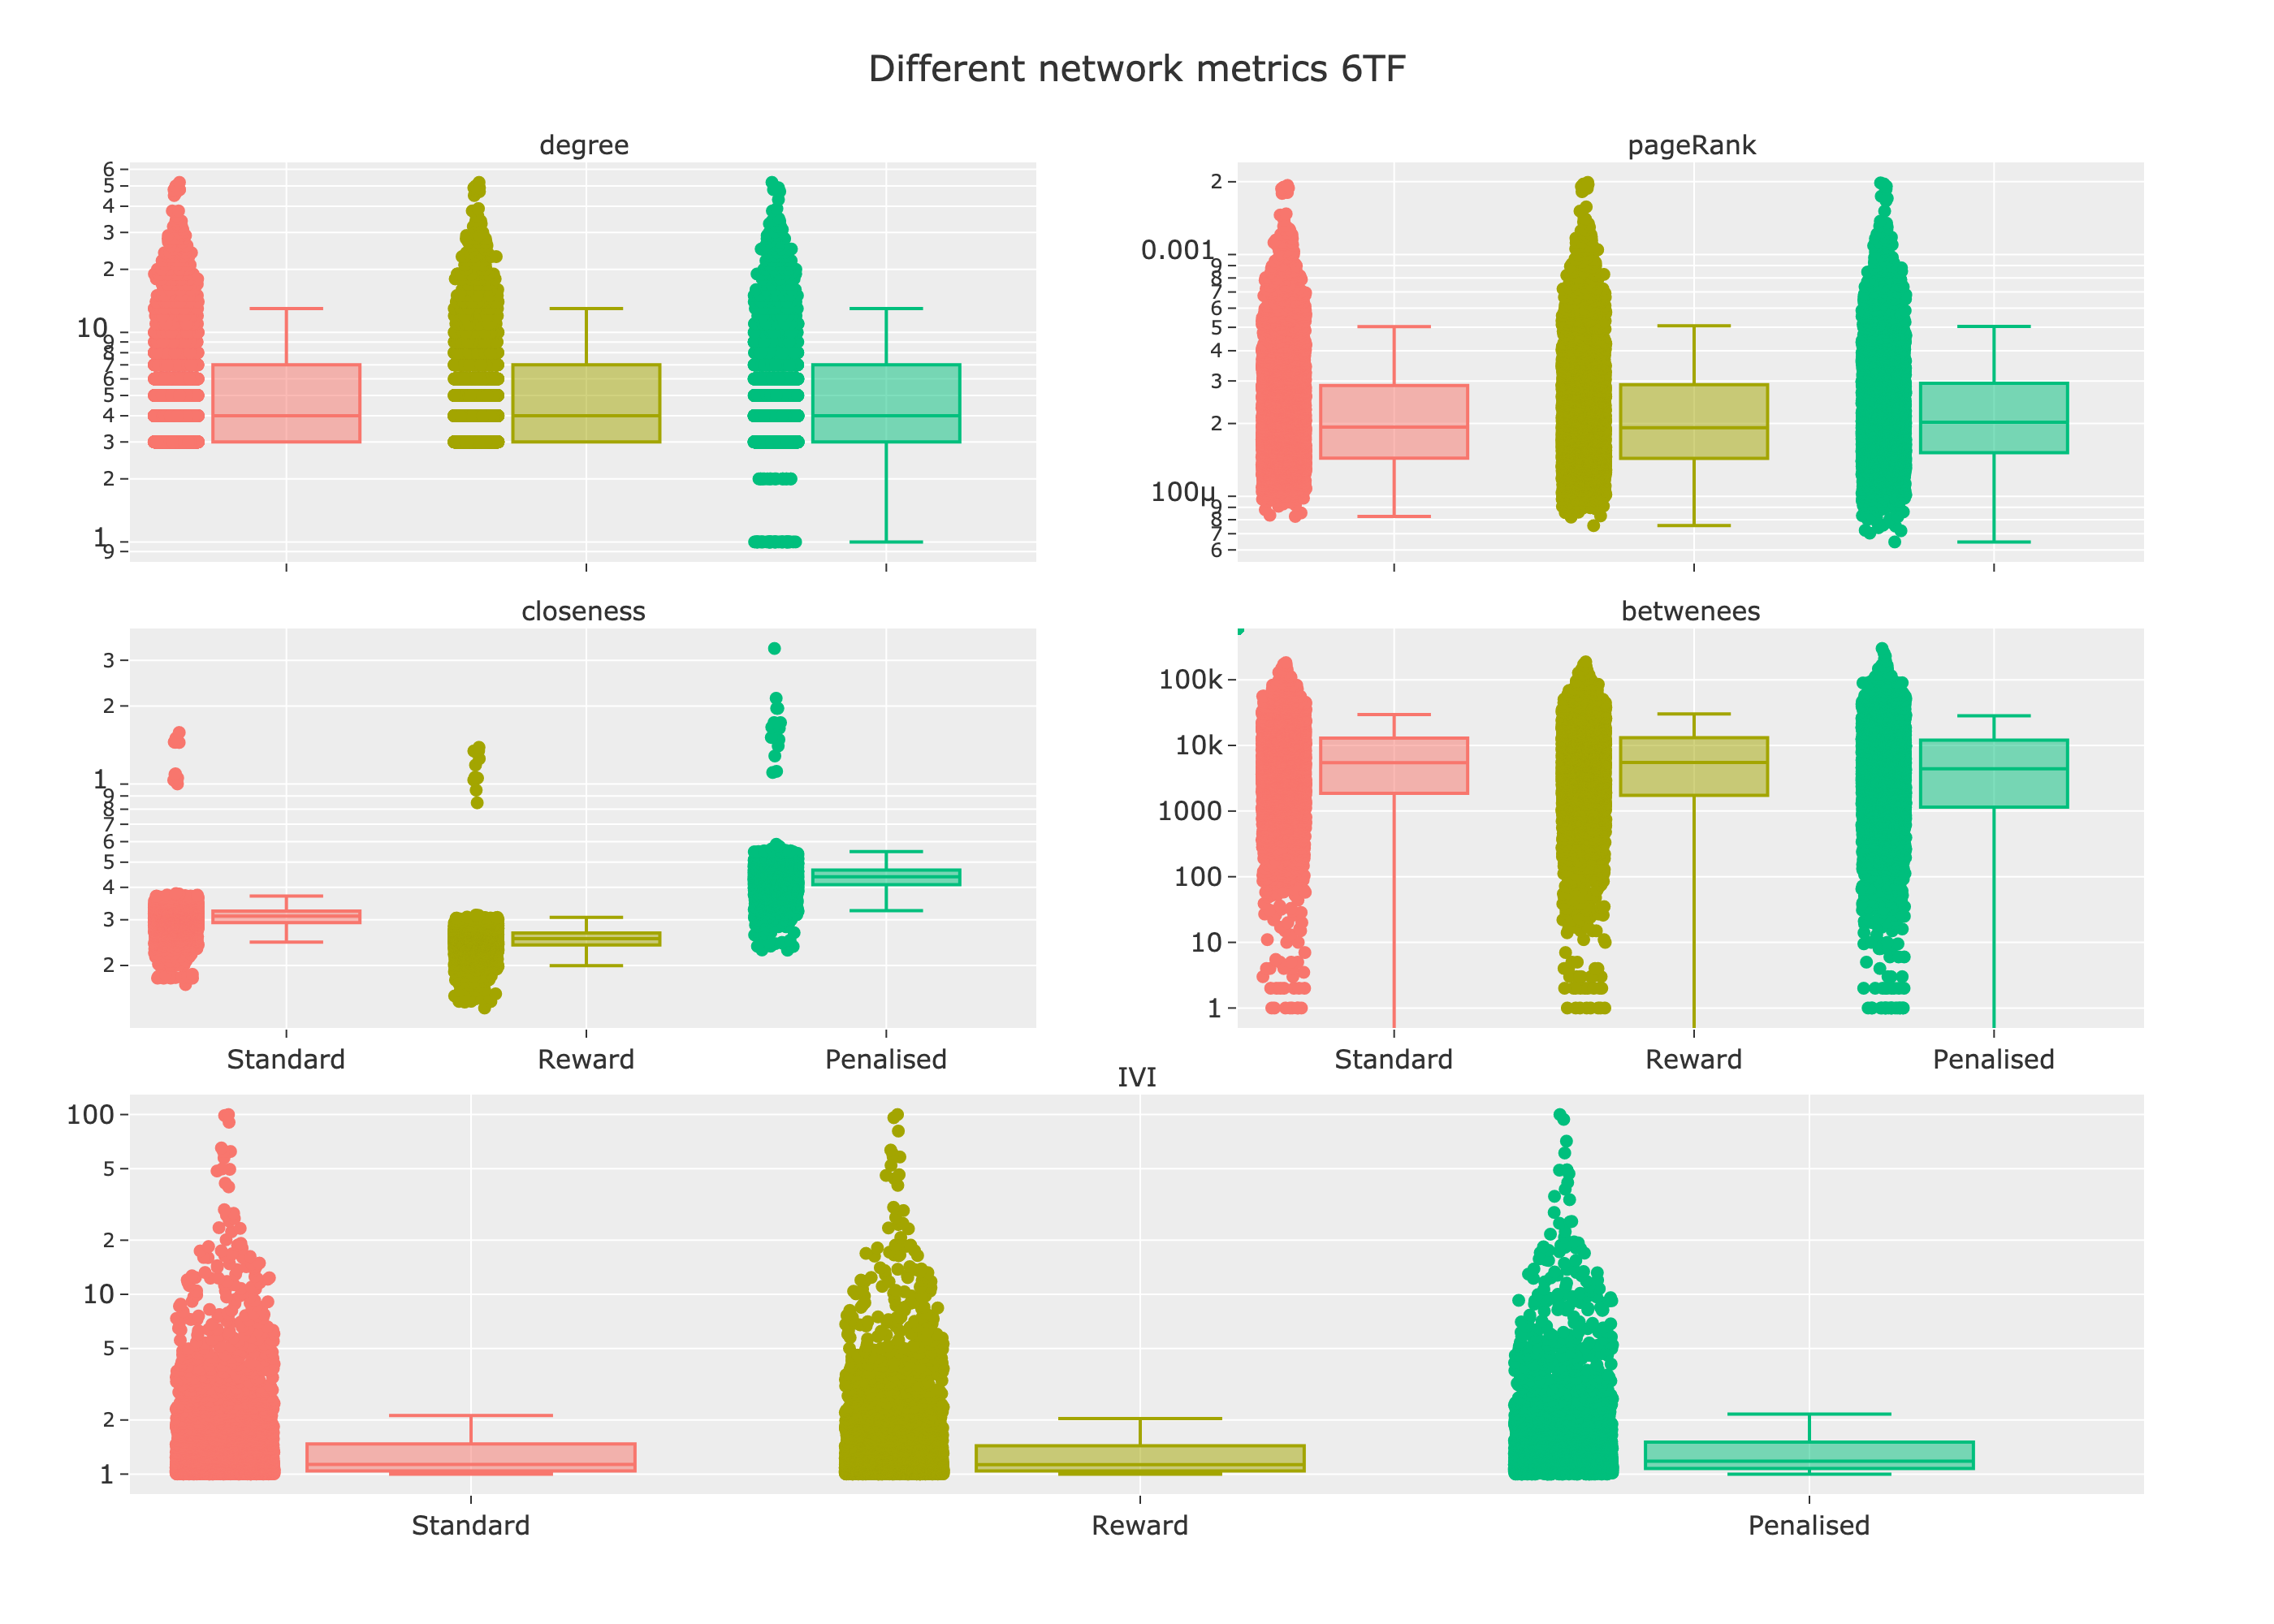
\includegraphics[width=1.0\textwidth,keepaspectratio]{Sections/Network_I/Resources/Tum_network/NetworkMetricsComp_6TF.png}
    \caption[Tum: centrality network metrics]{Network metrics for the tumour networks formed from 4K genes, 3 connections per standard gene and 6 for TFs with the different weight modifiers; standard (red), reward (mustard) and penalised (green). The y-axis represent is in log10 of the metric. Higher the degree or pageRank values more important the network is to the network, smaller values of closeness metric indicates that the vertices are closer together, while higher values of betweenness means that a node serves as a key bridge between other nodes. Higher values of \acrlong{ivi} indicates the node has a large influence both locally and globally to the network. Overall, trengthening the weights brings nodes closer together, while penalising spreads the vertices further apart.  }
    \label{fig:N_I:net_metrics_tum}
\end{figure}

% Describing the network
The graph metrics introduced in \cref{s:lit:net_metrics} are used to describe the networks built from the gene expression of the TCGA samples, where scores for the standard (red), reward (mustard) and penalised (green) network are shown in \cref{fig:N_I:net_metrics_tum}. Overall, the score exhibit the same trends across the three networks but the effects of the weight modifiers can be noticed in some of the metrics, closeness or degree.

% Difference in the penalised network
In the box plot for the degree metric, the distributions for the standard and reward network appear identical but without any significance (\acrshort{mw}: 8062709.0, p-value: 0.53541), both with a lower fence and a minimum value of 3. However, the penalised network contains several nodes (39) with values of 1, and its lower fence is at 1. This indicates that some genes are isolated in the penalised network. 

A similar trend is observed in the closeness metric across the networks, where all three graphs have a group of nodes with higher values ($>$0.7),  indicating that these nodes are further apart compared to the rest. This trend is more discernible in the penalised network, which has 17 versus 12 nodes with values more than 0.7. This can be explained by how the penalised modifier reduces the edge weights of the mutated genes closer to 0, as shown in \cref{fig:N_I:modifiers}.

% Reward modifiers
Rewarding the mutated genes with stronger connections has a noticeable effect on the network, though it is less pronounced than the effect of the penalised modifier; see \cref{fig:N_I:net_metrics_tum}. The largest difference is seen in the closeness metric (\acrshort{mw}: 5806.7421 p-value: 0.0), where the median and lower fence values for nodes in the reward network are $0.25$ and $0.19$, respectively, compared to $0.30$ and $0.24$ in the standard network. This indicates that the nodes in the reward network are significantly closer together compared to those in the standard network.

% Main conclusion - effects of the reward and penalised
The two weight modifiers applied have an effect on the constructed graphs, as shown by the metrics in \cref{fig:N_I:net_metrics_tum}. Strengthening the weights brings nodes closer together, while penalising spreads the vertices further apart. 

% Mutation in networks
\subsubsection*{Mutations in networks} \label{s:N_I:mut_rep}

% Why are we doing this analysis - understand the mutation burden reprsentation
To further understand how the network is affected by the weight modifiers it is important to check the presence of the mutation burden (i.e. the number of samples with the mutated gene) across the genes in the network. There are $\approx30K$ genes in the MIBC cohort from TCGA from which less than a half ($\approx13K$) are considered expressed by the aggressive filtering where more than 4 samples have TPM values larger than $0.5$. It is worth noting that the mutated genes in the TCGA contain only non-synonymous changes (Frameshift, Missense and Nonsense) meaning that all the includes may have a potential effect on the protein. 

% Commenting the trends
From the $\approx13K$ genes there are $\approx10K$ genes which are mutated at least once but then as the mutation count is increased there are fewer genes represented as seen in \cref{fig:N_I:mut_rep_tum}. The same trend can be noticed for TFs genes initially being 1027 genes in all the expressed genes, from which about a quarter (265) are mutated; the bottom bar plot in \cref{fig:N_I:mut_rep_tum}.

% Implications
The striking aspect of the \cref{fig:N_I:mut_rep_tum} is the inverse relationship of the number of abnormal genes with the mutation burden, e.g., for mutation burden $>=10$, there are 386 of the 4000 genes initially used for building the network ($\sim10\%$) and 36 out of the 265 TFs ($\sim14\%$). The trend can be noticed in both all the 4000 genes and the TFs but the latter has a higher representation of the mutated genes, see \cref{fig:N_I:prct_mut_rep_tum}. Of particular importance is the dysregulation of TF which up or down regulated of others gene expression.

\begin{figure}[!htb]    
    \centering
    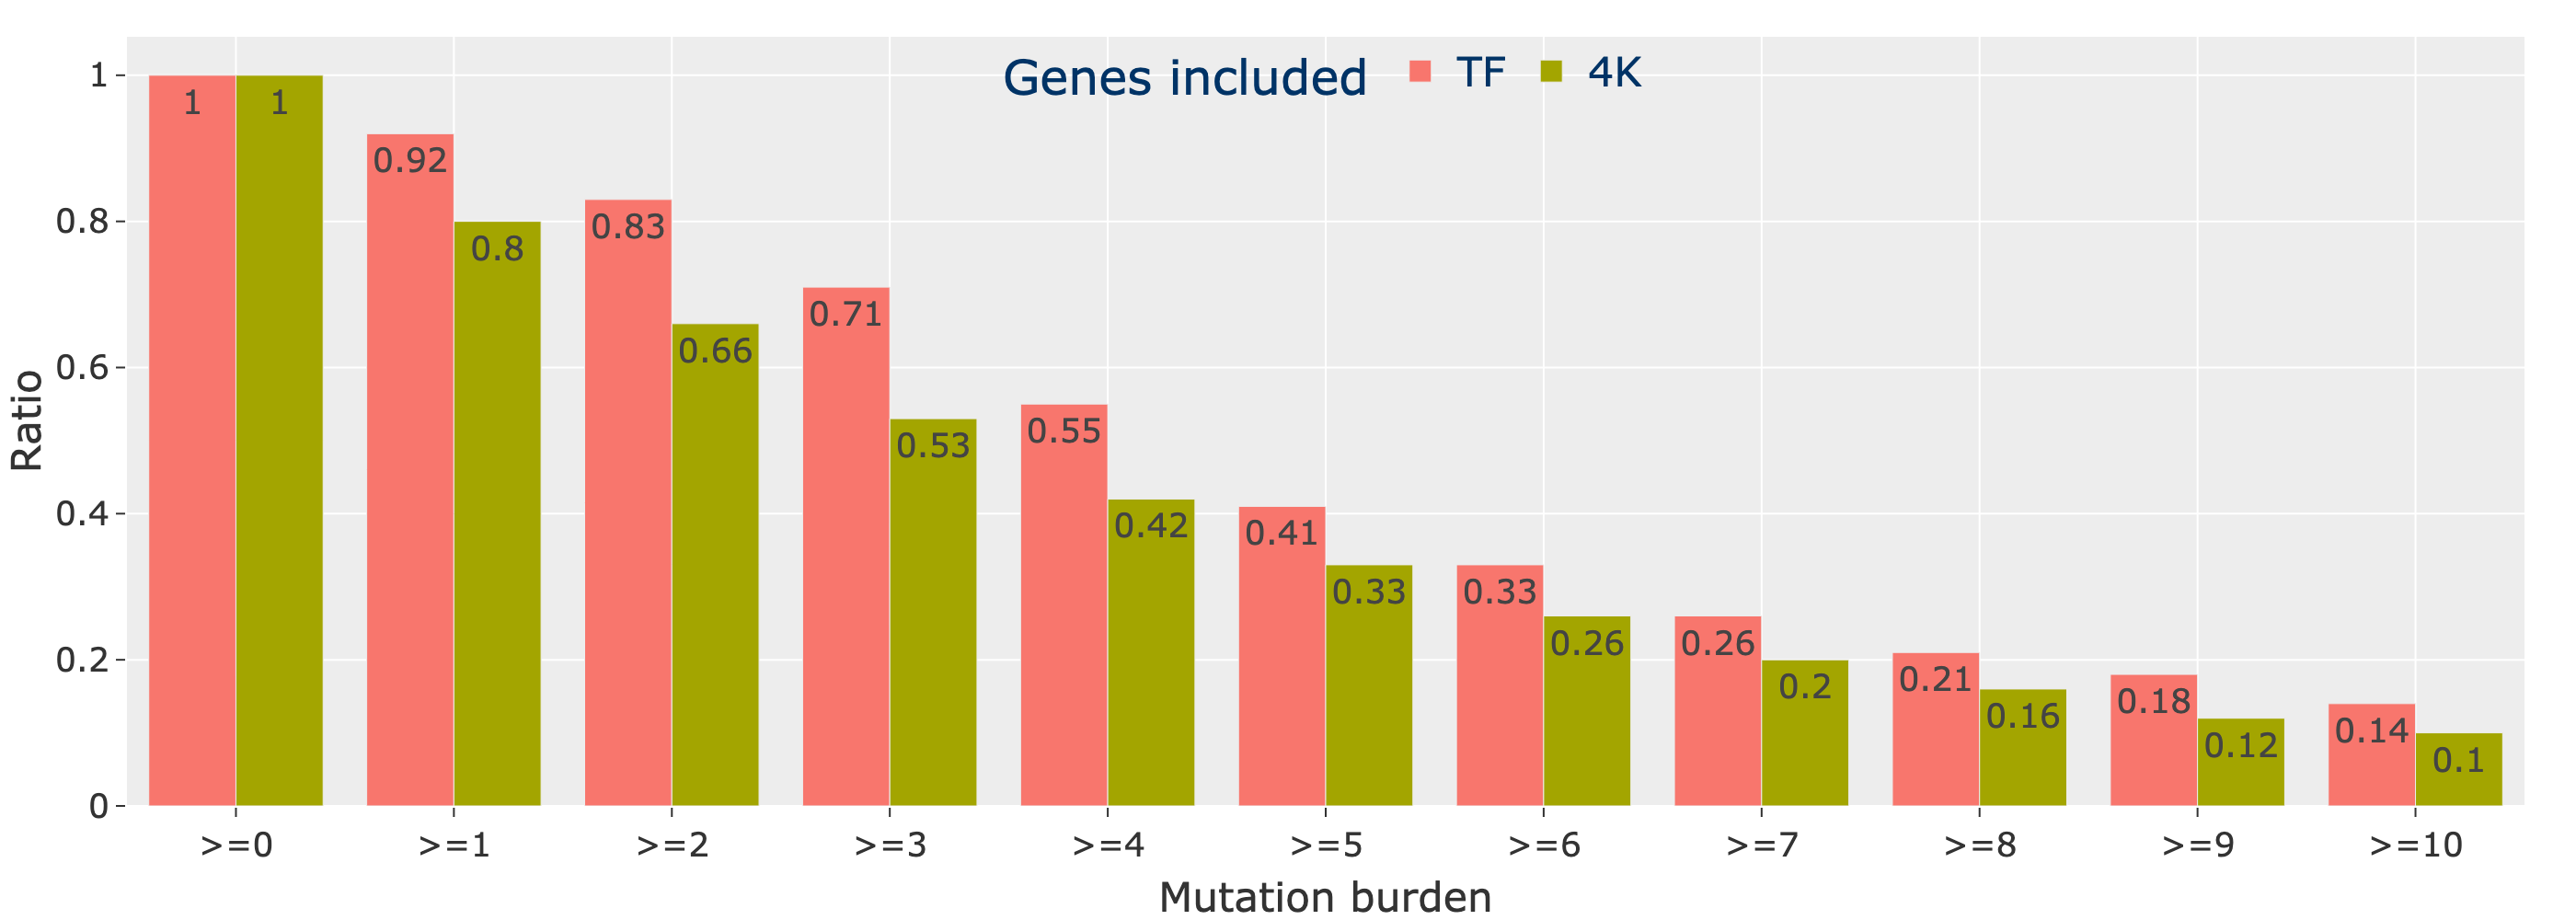
\includegraphics[width=1.0\textwidth,keepaspectratio]{Sections/Network_I/Resources/Tum_network/MutTF_representation_4K_TF_prct.png}
    \caption[Ratio of TF genes included by ModCon as mutation burden increases]{Ratio of TF genes as the mutation burden increased for both all 4000 genes and only the 265 TFs included in the 4000 most varied genes. It shows that that the TFs included the network are generally consists of mutated genes.}
    \label{fig:N_I:prct_mut_rep_tum}
\end{figure}

% Linking it back to the weight modifiers
With a low representation of the mutated genes the weight modifiers might have a limited impact into the network and the MIBC stratification. This is not so explicit in the tumour networks but it is present in the graphs derived in the tumour derived graphs.

% Leiden stratification
\subsection{Leiden and MIBC stratification} \label{s:N_I:tum_stratification}

% Introducing the algorithm and why I am doing this
% Justify the use of K-means with K = 6
The Leiden algorithm, with Modularity Maximisation set as the quality function, was applied ten times to study the variability of the community detection algorithm. The three graphs: standard, reward and penalised, were built from the 4,000 most varied genes, with a minimum degree of 3 for standard genes and 6 for TFs\footnote{See \cref{s:N_I:sel_tfs} for the experiments and data that support the configuration of 6 edges per TF.}. After applying ModCon to the important genes from the network, K-means clustering (K=6) was performed on the MEV values to identify MIBC subtypes. The group size of 6 was chosen to maintain consistency with previous findings (i.e., the clustering analysis from \cref{s:clustering_analysis}), where 6 subtypes of MIBC were identified, and to avoid introducing additional variables into the comparisons\footnote{A more in-depth clustering analysis is performed on the MEV scores for the P0 network in \cref{s:ap:p0_clustering}.}. The goal of this set of experiments was to understand the changes in the MIBC subtypes resulting from the reward and penalised networks.


% Talk about the number of communities
\paragraph*{Effects on Leiden}


The Leiden algorithm tends to find more communities in the standard network, with a maximum of 26 and a third quartile of 25, compared to 25 and 24 in the penalised network, as shown in the left box plot in \cref{fig:N_I:tum_leiden_modifiers}. The reward network contains the smallest number of groups across the three networks, with a median value of 23 compared to 24.5 (standard) and 24 (penalised). However, it is less varied, with the median value equal to the first quartile. Overall, there is a small non-significant difference (\acrshort{kw}:  3.3047, p-value 0.1915) in the number of communities found by the three networks, and the Leiden algorithm is more stable in the reward network, while it finds more communities in the standard network.

% Modularity Maximisation
The Modularity Maximisation score measures the quality of community separation, thus evaluating the performance of the Leiden community detection algorithm; see \cref{s:lit:comm_detect} for a more detailed overview. The standard and reward networks have higher but Modularity scores compared to the penalised network, suggesting that the communities found in these graphs are better separated but there is no significant difference\footnote{Standard and Penalised (\acrshort{mw}: 0.496, p=0.481); Reward and Penalised  (\acrshort{mw}: 3.304, p=0.100)}, as shown in the right box plot in \cref{fig:N_I:tum_leiden_modifiers}. The standard network has the lowest variance in Modularity scores contrasting the stability of Leiden in the reward network. The penalised network performs the worst according to Modularity Maximisation score, which is consistent with the results from the network metrics explored in the previous section, see \cref{s:N_I:tum_describe}.

% Introduce the Sankey plot
Overall, the two top box plots shows that the weight modifiers have an effect on the community detection algorithms and on the MIBC stratification are shown on the bottom Sankey plot; \cref{fig:N_I:tum_leiden_modifiers}. It is worth mentioning that the top performing network by Modularity Maximisation is selected for each of the network types and are then compared with classification in the literature (TCGA - \citep{Robertson2017-mg} and Consensus \citep{Kamoun2020-tj}) and our previous classification using the clustering analysis in \cref{s:cs:right_config}. 


\begin{figure}[!t]    
    \centering
    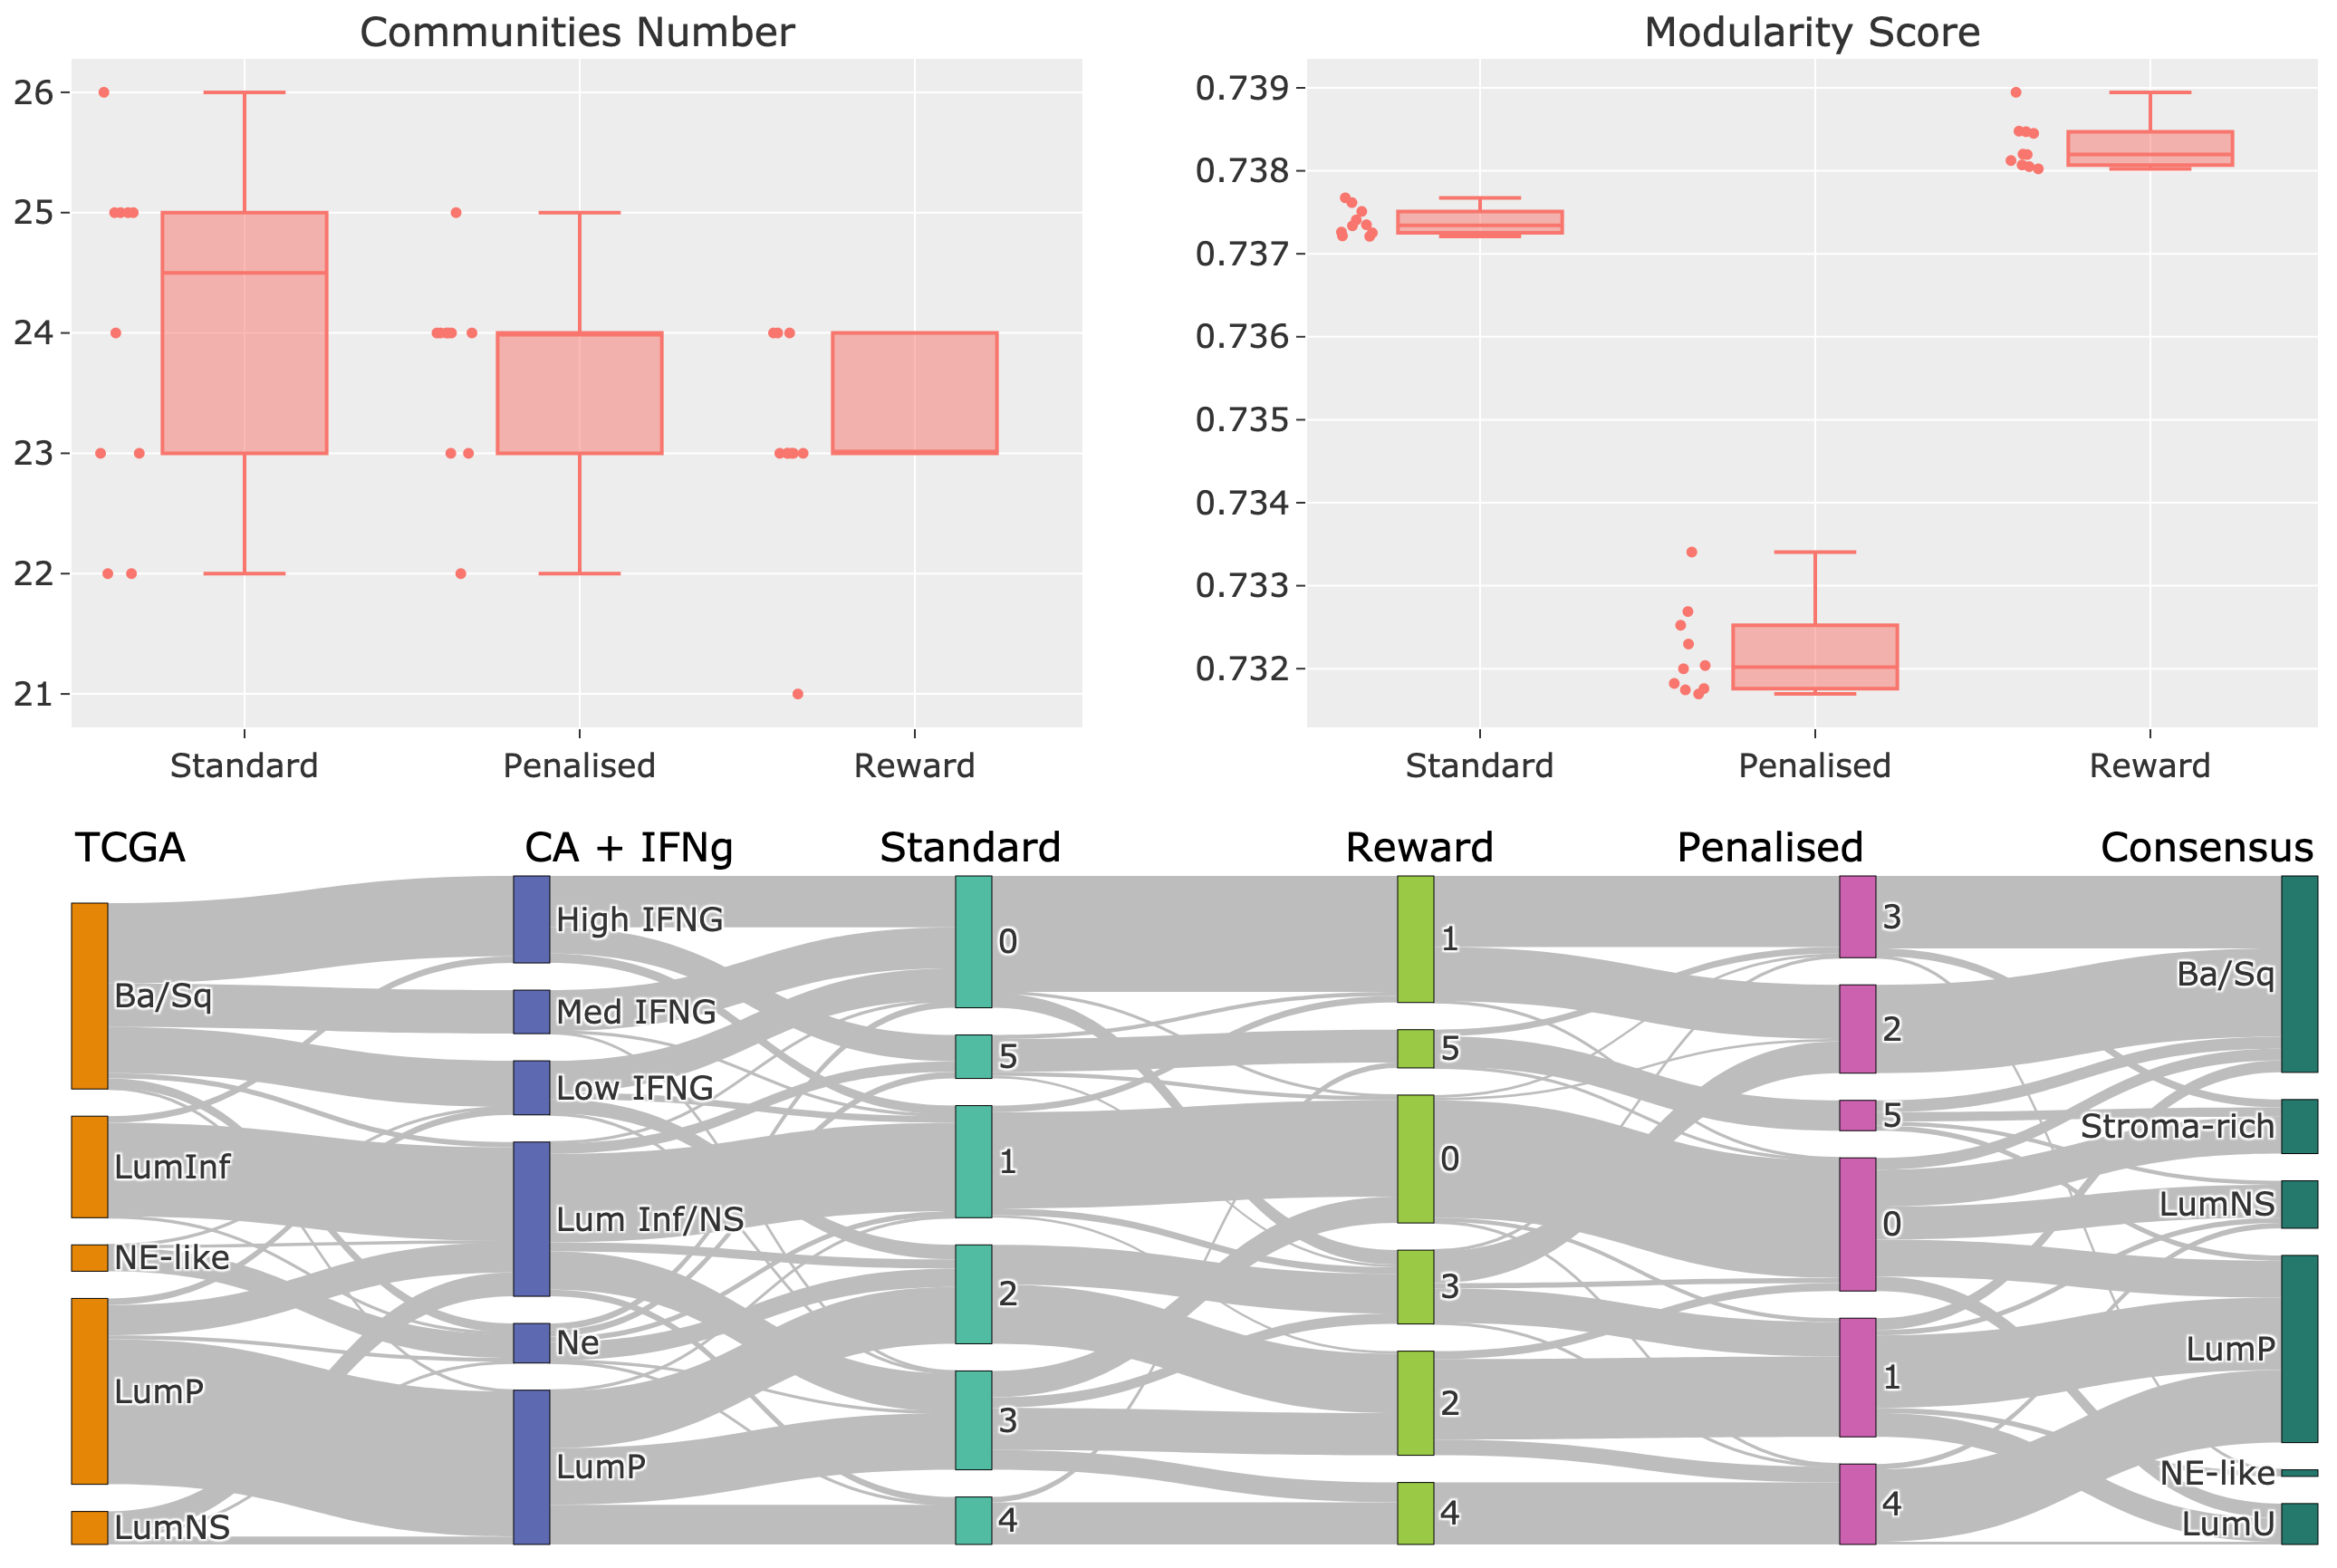
\includegraphics[width=1.0\textwidth,keepaspectratio]{Sections/Network_I/Resources/Tum_network/LeidenMetrics_Sankey_TF-6.png}
    \caption[Tum: Leiden metrics]{On the top are displayed the community size and Modularity Score. The two metrics used to asses effects of the weight modifiers (standard, reward and penalise) to the Leiden algorithm. At the bottom the Sankey plot displays comparison between the MIBC subtyping derived from the different standard classifiers (TCGA \citep{Robertson2017-mg} and consensus \citep{Kamoun2020-tj}), the previous developed subgroups with the cluster analysis \cref{s:clustering_analysis} and the three different networks. The figure shows that the weight modifiers affect the communities found through Leiden and exhibit different subtypes compared to previous classifications.}
    \label{fig:N_I:tum_leiden_modifiers}
\end{figure}

% Comment on the Sankey
% - Different subtypes but keeping the two main signal: Basal/Luminal across the classification
% - Have some Basal groups
\paragraph*{Effects on MIBC stratification}


All three networks show different clusters compared to the previous classifications, including our own, which immediately suggests that the network pipeline from \cref{fig:N_I:network_pipeline} has the potential to identify new groups. Although the two main 'signals' of Basal and Luminal subtypes are preserved across the clusters identified through the network pipeline. It is also important to note that the Luminal groups are split into smaller subgroups compared to the clustering analysis from \cref{s:clustering_analysis}. 

% Commenting on the basal
The basal subtypes with different immune response (Low/Med/High IFNG) are not as clearly defined as in the previous clustering analysis, there is still some separation among these samples. Group 5 which predominately contains High IFNG and Luminal Infiltrated samples, it is commonly found across all three network, suggests that it contains the sample with a high infiltration of either immune or stroma cells as many samples were previously classified stroma-rich (TCGA and Consensus). While the High/Med and Low IFNG samples are clustered together in the standard and reward networks, the samples previously classified as Low IFNG are combined with neuroendocrine ones in the reward network and with Luminal samples in the standard and penalised networks. This suggests that the reward network might better isolate the undifferentiated samples\footnote{see the biological interpretation of the Basal groups from \cref{s:cs:basal_interp}}.

% Linking the difference shown by the weight modifiers
Concurrently, there is difference in the MIBC subgroups found by the three network types suggesting that the weight modifier have an impact to the tumour's stratification. In addition, the two weight modifier strategies exhibit different MIBC groups with the reward network being closer to the standard graph while the penalised network being the most different from the other two. This can be seen best in the split of the Ba/Sq group (consensus) by the penalised network, while the standard \& reward do not discriminate between the two groups. As mentioned earlier all three networks find a small group of Stroma/Basal (5).

Overall, the stratification shown in \cref{fig:N_I:tum_leiden_modifiers} shows the potential of the Network approach of finding different groups from previous stratification work, including the clustering analysis from the previous section \cref{s:clustering_analysis}. The figure also indicates that the weight modifier have an effect on both the Leiden algorithm and the MIBC stratification, where the groups derived with reward closer to the ones from standard, and penalised exhibited larger differences. The graphs do not find the three different immune Basal groups found previously but there is a consistent small group, 5, which might be related with cell infiltration, thus showing the potential of the network approach to find new biological relevant groups.


% Nonetheless, there is little difference between the networks suggesting that the weight modifiers do not have a high impact on MIBC stratification with K-means (K=6).

% Further commenting on the Sankey
% As it was mentioned earlier that the two main Basal and Luminal 'signals' are found in the the subtypes derived from the three networks. The \acrfull{lump} is split into two smaller groups across with varying sizes, while the Luminal Infiltrated (from the previous clustering analysis) is also consistently found by the three networks.

% There are more changes in the Basal (TCGA/consensus) and \acrfull{ne}. The Standard and Reward are consistent in finding the same 3 groups (\textbf{0, 3, 5}) where \textbf{1/0} is a mixed of LumInf/NS and High IFNg, \textbf{4} is mainly Low IFNG and a few NE samples while \textbf{2} is a combination of High and Medium IFNg. This may suggest that cluster 4 represents the tumours which are more basal (de-differentiated), while \textbf{5} the tumours with high infiltration and immune response and cluster \textbf{2} the samples between the two. In the Penalised network sub-grouping the cluster \textbf{5} remains the same, but \textbf{4} and \textbf{1} are changed. The former contains more of the LumP and Low IFNG samples, while the latter hold most of the IFNG samples. This suggest that the Penalised network stratification perform worst.


% cluster analysis vs network gene selection
\subsection{Clustering analysis vs network gene selection} \label{s:N_I:cs_vs_gene_sel}

% Network as a gene selction
The network pipeline developed in this section can be thought as a sophisticated gene selection mechanism based on multiple data-types: gene co-expression, mutation and transcription factors. Specifically as the ModCon step from  \cref{fig:N_I:network_pipeline} picks the genes that have the highest connectivity (see \cref{eq:modcon}, which are then used for clustering analysis (through MEV). Similarly, in the previous chapter $\approx3K$ top most relative varied genes were used in the K-means clustering analysis. Therefore, there is a need to compare the two gene selection methods and to assess the differences.

% What's the comparison
The comparison is performed only using the TCGA's MIBC dataset to avoid gene expression differences introduced by the healthy samples. The network was constructed from the 5K most varied genes, no weight modifier and the minimum degree for TFs  was set to 6\footnote{The Selective Edge pruning experiments from \cref{s:N_I:sel_pruning} showed diminished returns from allowing more than 6 edges per TF.} and 3 to the standard genes. For a network formed of 5K genes, the ModCon (=100 for each community) selects in total $\approx2.8K$ genes which is comparable with the 3K most relative varied genes. Note, in the cluster analysis work from \cref{s:clustering_analysis} 3500 genes were used. So, the network size was increased and the number of genes selected was reduced so that the gene sets are comparable.

\begin{figure}[!t]    
    \centering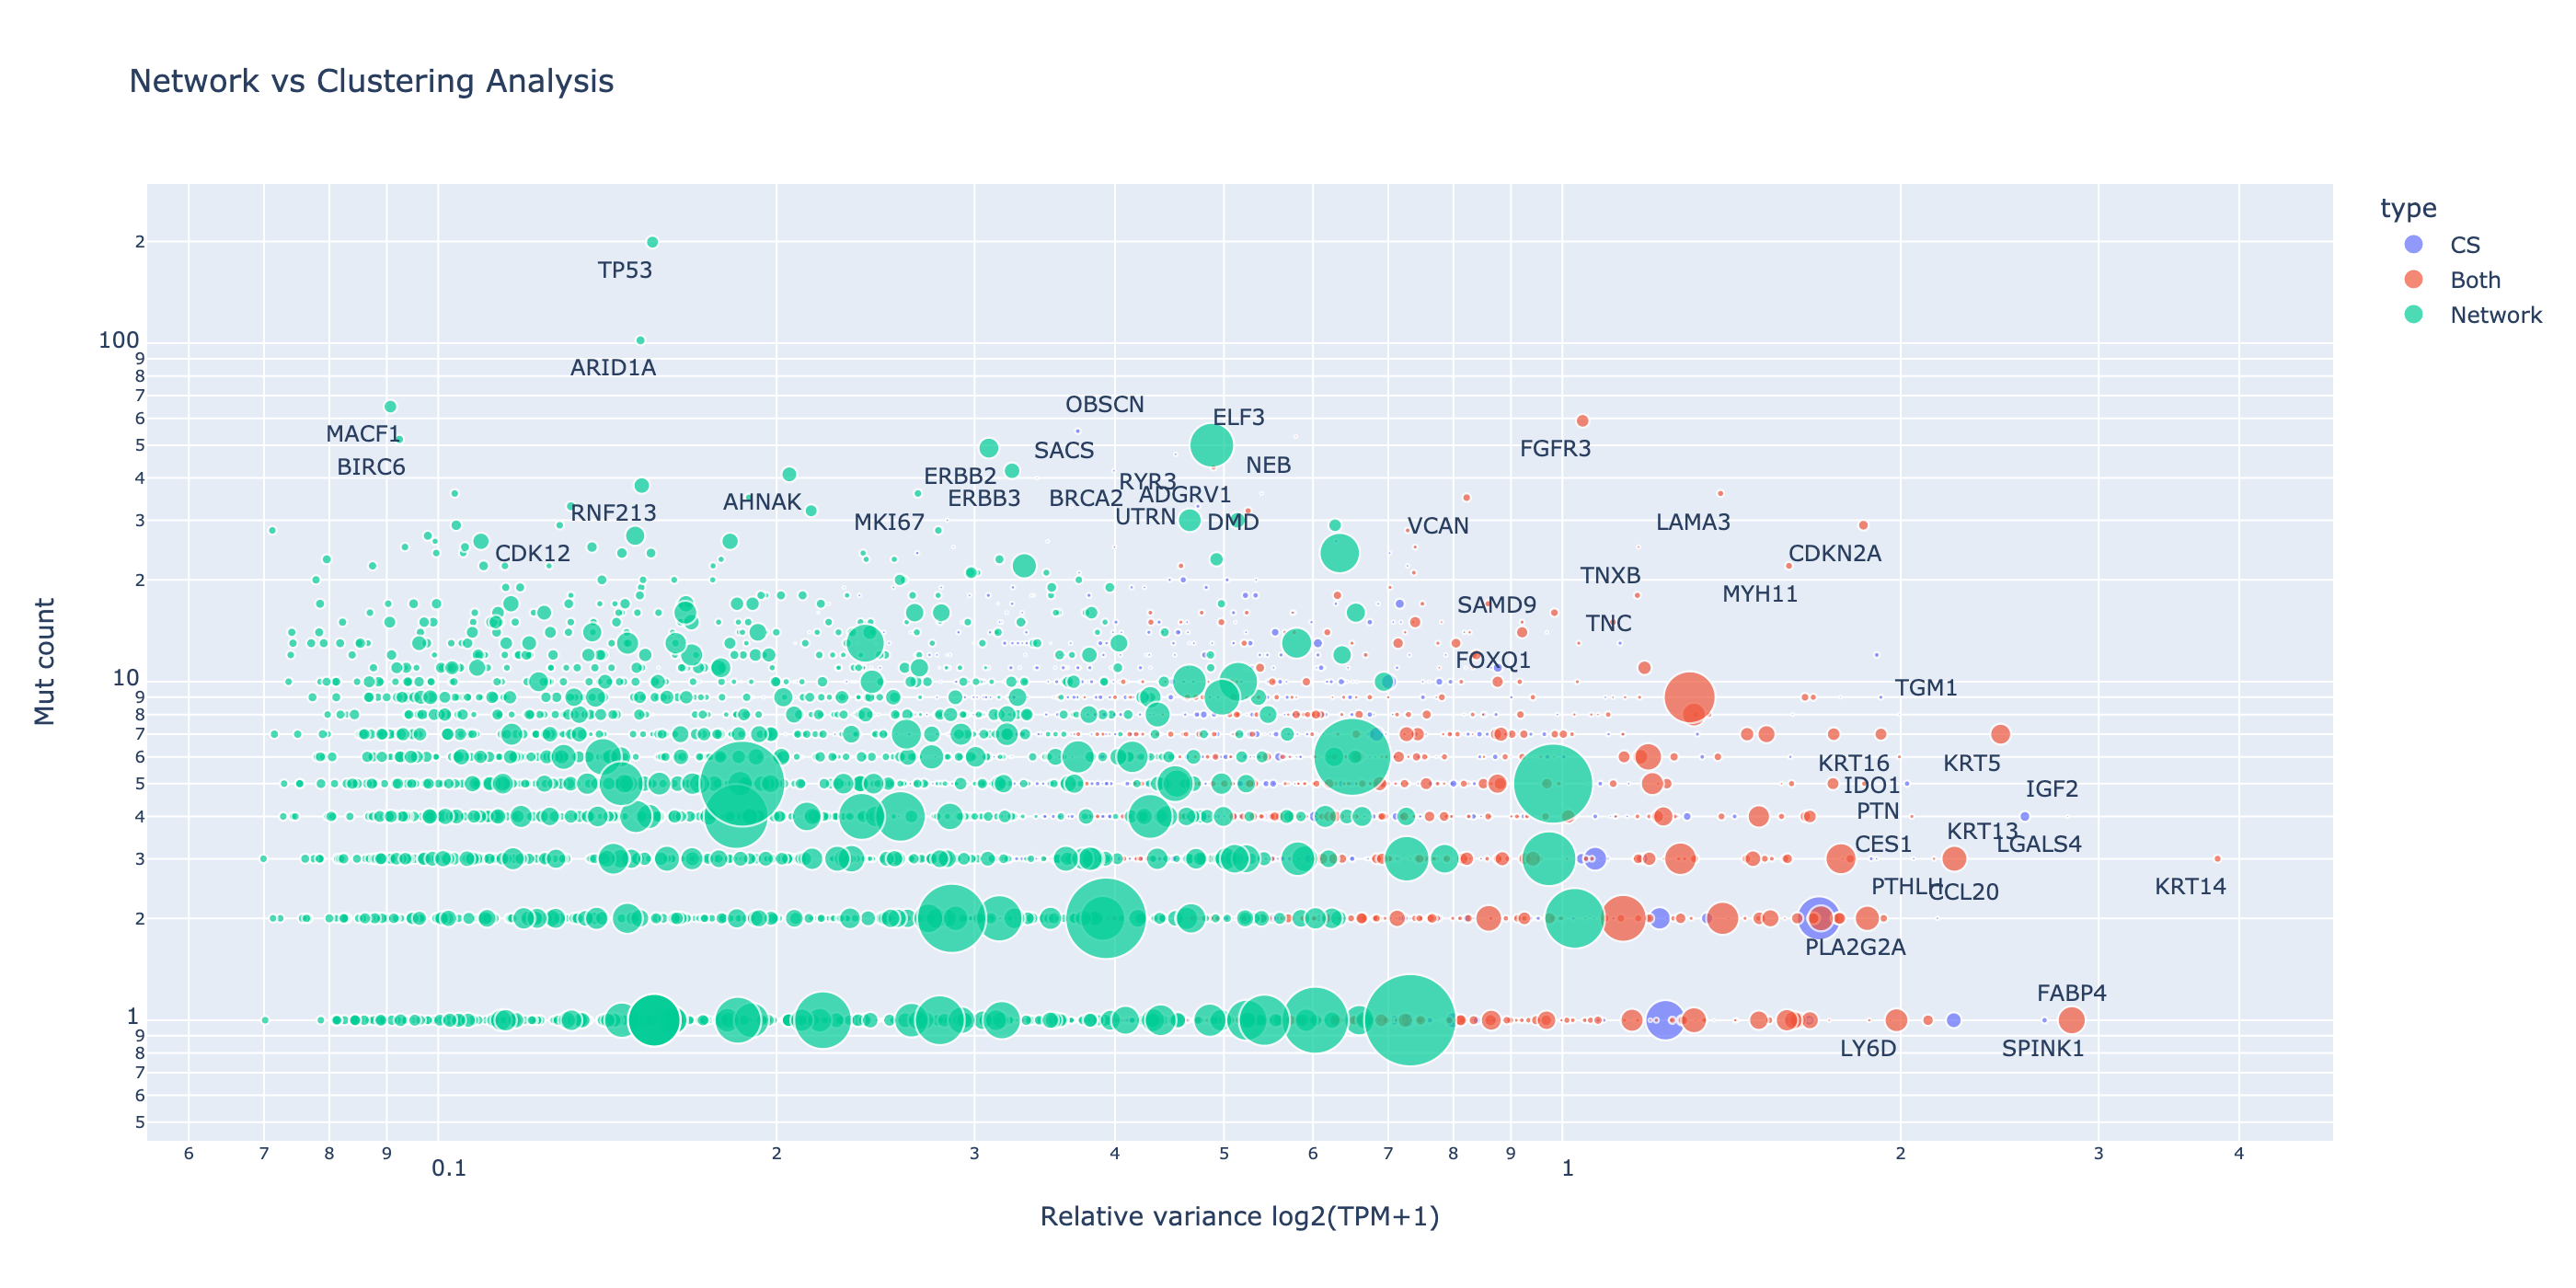
\includegraphics[width=1.0\textwidth,keepaspectratio]{Sections/Network_I/Resources/Tum_network/ClusteringAnalysis_vs_Network_3.png}
    \caption[Gene selection: network vs clustering analysis]{Network selection vs. Clustering Analysis. Red points are represented by the genes selected exclusively by the highest median standard deviation ratio, the green by the network and mustard by both approaches. The size of the points is the median expression of the genes across the TCGA sample. To avoid log values of 0 the mutations count were offset by one. Showing that the network approach selects genes that are not only highly varied but also have higher median expression and mutation burden.}
    \label{fig:N_I:network_ca_selection}
\end{figure}

% Interpret the results
Between the two sets of genes there are 2053 different genes and 747 shared which are all shown in the variance vs. mutation burden scatter plot from \cref{fig:N_I:network_ca_selection}. As expected the genes selected only by relative variance are skewed to the right picking the highly mutated genes that also have a high variance. By contrast, the network approach not only selects most of the varied genes but also some of the highest mutated genes despite having low variance. The points' size is relative to the median expression in the TCGA cohort and from the Figure \ref{fig:N_I:network_ca_selection} it can be seen that the canonical gene selection does not include the highly expressed genes as the network does.

This comparison shows the power of the network approach which selects not only the highly varied genes but also the ones that have consistent expression values and high mutation burden. This means that the graph method is capable of selecting genes with more diverse molecular properties compared to the other methods, which may lead to newer and different MIBC subgroups.

\subsection{Summary}

% Effect on the network metrics and communities
The two sets of experiments performed in this section suggest the potential of a network-based approach to stratify MIBC. The three different networks—standard, reward, and penalised—were validated using various network and community detection metrics \cref{fig:N_I:net_metrics_tum,fig:N_I:tum_leiden_modifiers}. Both analyses demonstrated that the weight modifiers affect both the nodes' properties (e.g., degree, closeness) and the Leiden algorithm.

% MIBC subtyping
The MIBC subgroups derived from the three networks differed from existing stratifications, highlighting the potential to identify new subtypes. Compared to the previous clustering analysis in \cref{s:clustering_analysis}, the networks were unable to identify the three Basal immune groups but showed promise for uncovering new biology, as evidenced by the identification of a small group, 5, which contained samples previously classified as Stroma. Additionally, the two different edge weight modifiers revealed distinct groups from each other and the standard network, indicating the effect of mutations in the network.

% Gene selection
Following this, the differences in gene selection between the Clustering Analysis and the network approach were explored, as depicted in \cref{fig:N_I:network_ca_selection}. This comparison shows that the network is capable of selecting genes with a wider range of properties. Genes with higher mutation burdens, greater magnitudes, and higher variance are selected by the network approach, while the standard approach tends to select only those with the highest relative variance.

Overall, the experiments in this section demonstrated the advantages of the network approach as a method for cancer subtyping and the effects of integrating mutation data by modelling edge weights. The following section will explore the data integration at network level.
